\begin{figure*}[h]
    \label{badandother}
  \begin{center}
    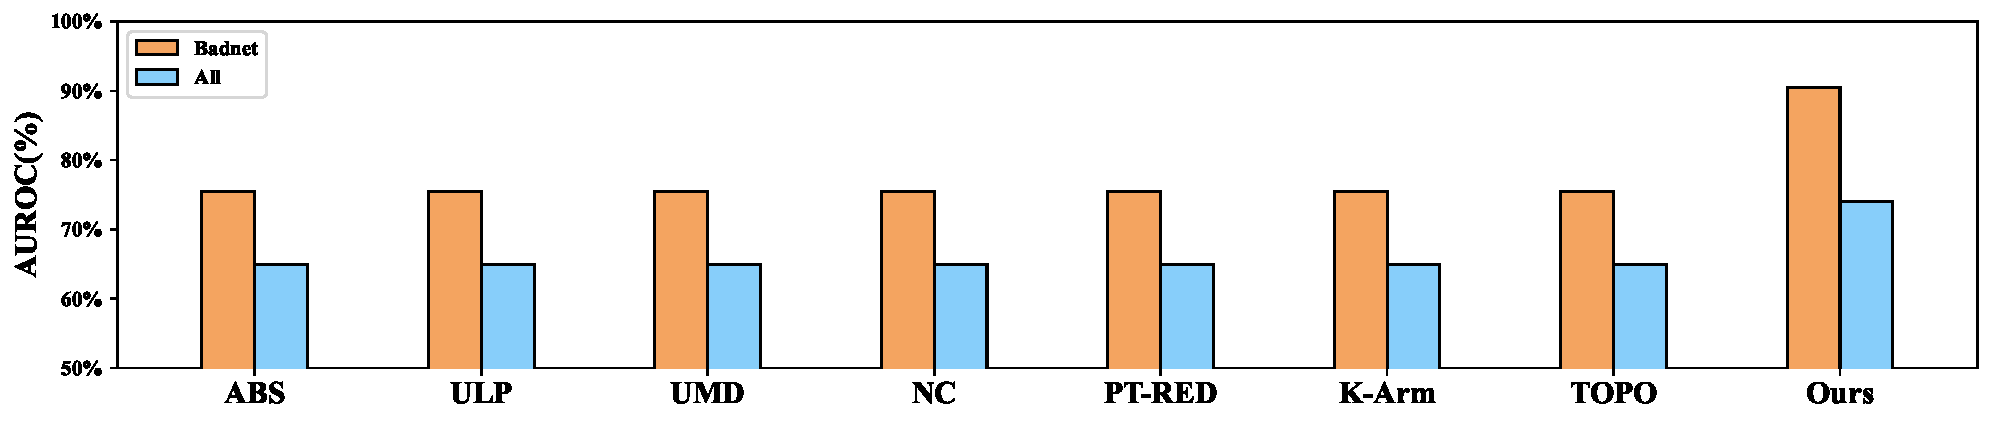
\includegraphics[width=1\linewidth]{Images/badnetvsothers.pdf}
    \caption{Comparison of Accuracy across different trojan scanning methods. The chart illustrates the performance of each method on BadNet (orange) versus all other attacks (blue) in our collection of 8 distinct attack methods. Notably, our method (TRODO) maintains a consistent performance across both BadNet and other attacks. This indicates a superior generalization capability compared to other \kian{(attack or scanning?)} methods, which display a marked preference and possible overfitting to BadNet, leading to reduced scanning ability on varied attack types. \kian{There is no ref to Fig 2 in the text. Also, why did you choose Badnet separate from all other methods? The conclusion written about this figure is also unclear.}}
    
    \vspace*{-4mm}
    \label{fig:motivate_fig}
  \end{center}
\end{figure*}